\documentclass{article}

% if you need to pass options to natbib, use, e.g.:
%     \PassOptionsToPackage{numbers, compress}{natbib}
% before loading neurips_2019

% ready for submission
% \usepackage{neurips_2019}

% to compile a preprint version, e.g., for submission to arXiv, add add the
% [preprint] option:
%     \usepackage[preprint]{neurips_2019}

% to compile a camera-ready version, add the [final] option, e.g.:
     \usepackage[final]{conducktors}

% to avoid loading the natbib package, add option nonatbib:
%     \usepackage[nonatbib]{neurips_2019}

\usepackage[utf8]{inputenc} % allow utf-8 input
\usepackage[T1]{fontenc}    % use 8-bit T1 fonts
\usepackage{hyperref}       % hyperlinks
\usepackage{url}            % simple URL typesetting
\usepackage{booktabs}       % professional-quality tables
\usepackage{amsfonts}       % blackboard math symbols
\usepackage{nicefrac}       % compact symbols for 1/2, etc.
\usepackage{microtype}      % microtypography
\usepackage[pdftex]{graphicx}

\title{Duckietown - Reinforcement Learning based on World Models\\ \textit{Duckietown - megerősítéses tanulás a World Models alapján}}

% The \author macro works with any number of authors. There are two commands
% used to separate the names and addresses of multiple authors: \And and \AND.
%
% Using \And between authors leaves it to LaTeX to determine where to break the
% lines. Using \AND forces a line break at that point. So, if LaTeX puts 3 of 4
% authors names on the first line, and the last on the second line, try using
% \AND instead of \And before the third author name.

\author{%
  conDUCKtors\\
  \textit{Máté Büki, Péter Zoltán Sánta, Gábor Tamás}\\
  Deep Learning in Practice with Python and LUA\\
  VITMAV45\\
  Budapest University of Technology and Economics \\
  2019/20/1
  %\texttt{hippo@cs.cranberry-lemon.edu} \\
  % examples of more authors
  % \And
  % Coauthor \\
  % Affiliation \\
  % Address \\
  % \texttt{email} \\
  % \AND
  % Coauthor \\
  % Affiliation \\
  % Address \\
  % \texttt{email} \\
  % \And
  % Coauthor \\
  % Affiliation \\
  % Address \\
  % \texttt{email} \\
  % \And
  % Coauthor \\
  % Affiliation \\
  % Address \\
  % \texttt{email} \\
}

\begin{document}

\maketitle

\begin{abstract}
  In our homework, we use a reinforcement learning framework to teach an agent to be able to follow the lane in the Duckietown Gym environment. The model our work is based on was named World Models \cite{worldmodels} and was published in 2018. The main idea of the model is to use a compressed representation of the observable environment instead of the raw image seen by the agent. The transformed observations are then passed to a recurrent neural network, which is responsible for the prediction of the next observation. Finally, using reinforcement learning, we train our agent according to the so called SAC policy.\newline
  \textit{Házi feladatunk keretein belül egy megerősítéses tanulás alapú, három komponensből álló modellt használva tanítottunk egy ágenst arra, hogy képes legyen az út követésére a Duckietown Gym szimulációs környezetben. Ehhez munkánk során a 2018-ban publikált ún. World Models\cite{worldmodels} modellt használtuk. A modell különlegessége, hogy nem az ágens által látott környezet nyers képét használja fel, hanem a környezet egy tömörített reprezentációját. Az így kapott, már transzformált megfigyeléseket továbbítja egy rekurrens neurális hálónak, amelynek feladata, hogy az ágens által a következő lépés során látott környezet transzformált formáját prediktálja. Végül az ágensünket megerősítéses tanulás segítségével, a rekurrens neurális háló kimenetét felhasználva tanítjuk az ún. SAC policy alapján.}
\end{abstract}

%%%%%%%%%%%%%%%%%%%%%%
\section{Introduction}
%%%%%%%%%%%%%%%%%%%%%%

Many of the algorithms in the field of artifical intelligence are inspired by how humans learn and think. Our brain is able to learn an abstract representation of the information it gets from our environment \cite{brain1}, \cite{brain2}. Our homework is based on a model called World Models\cite{worldmodels}, which mimics this behaviour. In their article, the authors present a new framework for facilitating the policy evolution in a reinforcement learning task. The main idea of their work is that they transform the environment seen by the agent into a latent vector, and the reinforcement learning algorithm is trained based on the already transformed reality. So the agent learns in its own world, hence the name of the model.


%%%%%%%%%%%%%%%%%%%%%
\section{Agent Model}
%%%%%%%%%%%%%%%%%%%%%

Our task was to implement the World Models\cite{worldmodels} (that has been already done for the OpenAI CarRacing environment) in the Duckietown Gym environment. In this chapter we briefly introduce the architecture of the model.

World Models has 3 basic components, depicted in figure \ref{fig:model}.

\begin{figure}
    \centering
    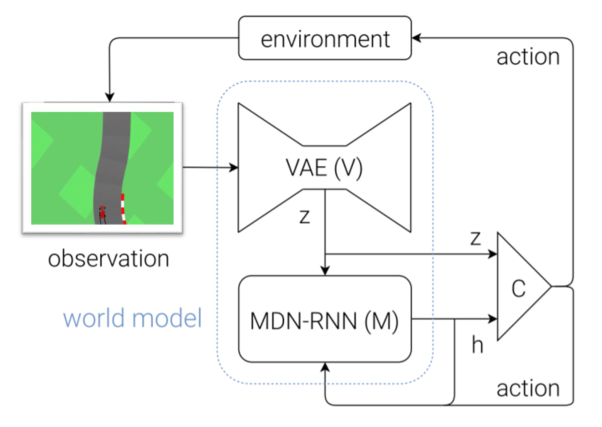
\includegraphics[width=0.6\textwidth]{world_models.png}
    \caption{Components of World Models}
    \label{fig:model}
\end{figure}

\subsection{Vision (V)}

 The Vision model is a simple Convolutional Variational Autoencoder (VAE) \cite{vae1}, \cite{vae2} which takes an observation (2D image) from the environment and encodes it into a latent vector $z$ of size 64.

The architecture of the VAE network is shown in figure \ref{fig:vae}.

\begin{figure}
    \centering
    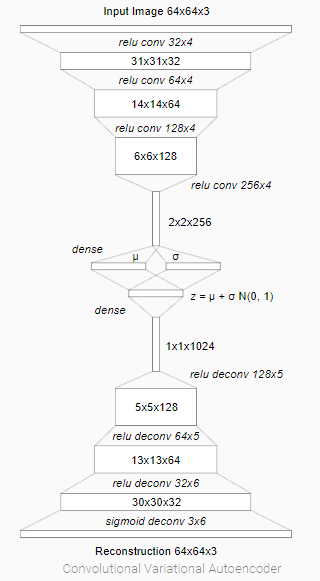
\includegraphics[width=0.4\textwidth]{VAE.png}
    \caption{Architecture of the VAE network}
    \label{fig:vae}
\end{figure}

\subsection{MDN-RNN (M)}
The second building block of the model we used is an LSTM\cite{lstm} recurrent Neural Network with Mixture Density Network\cite{MDN}. It takes the latent vector $z$ from the vision module, the previous action $a$ chosen by the controller and the previous hidden state $h$ of itself. Similarly to the vision module, its goal is to capture a latent understanding/observation of the environment by predicting what would the next $z$ look like.

The architecture of the Memory RNN network is shown in figure \ref{fig:rnn}.


\begin{figure}
    \centering
    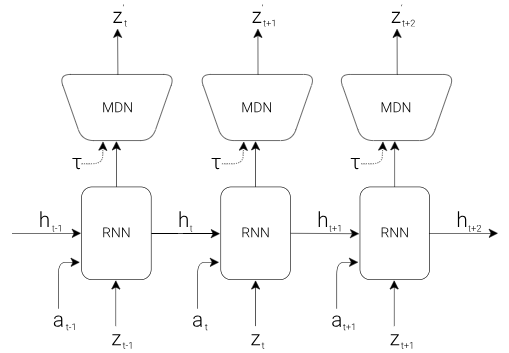
\includegraphics[width=0.4\textwidth]{RNN.png}
    \caption{Architecture of the Memory RNN network}
    \label{fig:rnn}
\end{figure}

\subsection{Controller (C)}
In the original implementation it was a simple single layer linear model which maps the vision module’s observation $z$ and the memory module’s hidden state $h$ to an action $a$ at each time step. The output is an action-vector (numpy array) of size 2 containing the quantitative representation of the velocity [-1.0 to 1.0] and the angle of the steering wheel [-1.0 to 1.0].
Instead of the simple linear model, we used the so called SAC reinforcement learning policy \cite{sac}. SAC uses entropy regularization and is trained to maximize a trade-off between expected return and entropy. Entropy is used to describe the randomness in the policy. A higher value of entropy leads in more exploration, which can accelerate the learning process.

%%%%%%%%%%%%%%%%%%%%%%%%
\section{Implementation}
%%%%%%%%%%%%%%%%%%%%%%%%

In our homework, we used the Duckietown Gym \cite{gym_duckietown} environment. Gym \cite{gym} is a toolkit for developing and comparing reinforcement learning algorithms. It supports teaching agents everything from walking to playing games like CarRacing or Pacman. Duckietown is a playful learning experience for state-of-the-art robotics and AI. It makes it possible to develop and test autonomous driving algorythms with Deep Learning in a joyful sandbox environment. To make the development easier, the Duckietown Foundation published the Duckietown Simulator based on the OpenAI Gym environment.

Modifying the structure of the model presented in \cite{worldmodels} was out of the scope of our homework. Our goal was to modify an already existing PyTorch implementation of World Models\footnote{https://github.com/ctallec/world-models} so that we can apply it in Gym-Duckietown.

\subsection{Data preparation}
We have created a dataset of 100 training, 50 testing and 20 validation rollouts. A rollout consists of four arrays, 

\subsection{Training the model}
Since our model has three components, we had to train it sequentially. In the first step, the VAE network was be trained independently in the following way:
\begin{enumerate}
    \item The network takes an image with a size of (640 x 480 x 3) as an input.
    \item A convolutional network creates a so called $z$ vector of length 64 as a compressed representation of the input image.
    \item A deconvolutional network then takes the $z$ vector as input and generates a (640 x 480 x 3) sized image as an output.
    \item Finally, the VAE network computes the loss based on the similarity of the input (original) and the output (generated) images. If the two images are quite similar, that means that the VAE learned to compress images efficiently into a vector of length 64.
\end{enumerate}

Note that the deconvolutional network will only be used during training, after that it will be ''deactivated''.


Before making a step forward, we will first fix the parameters of the VAE (we do not want it to train any more). Then the RNN takes two inputs in every step: the current $z$ vector from the VAE and the previous action $a$ chosen by the controller.

During the training of the RNN, we will use a simple random number generator (that generates two numbers in the range of [-1.0, +1.0]) to simulate the controller (due to the fact that it will not have been trained yet). The output of the RNN is the predicted $z$ value of the next step ($z+1$), so that the loss will be calculated based on the similarity of the current output of the RNN and the input from the VAE in the next step.

Finally, we will train the controller, but before that, we will first fix all the parameters of both the VAE and the Memory networks.


The controller takes two vectors as input, one from the VAE (the current $z$ vector) and one from the Memory (the hidden $h$ vector) and generates an action $a$ as an output.

Based on the action of the controller, the environment generates a reward (a float number) that indicates how good decision the controller has made. The aim of the controller is to maximize the reward it gets.


%%%%%%%%%%%%%%%%%%%%%%%
\subsection{Evaluation}
%%%%%%%%%%%%%%%%%%%%%%%

%%%%%%%%%%%%%%%%%
\section{Summary}
%%%%%%%%%%%%%%%%%



\subsubsection*{Acknowledgments}

We wish to acknowledge the help provided by Róbert Moni, who has guided us throughout the semester.

\section*{References}


\small
\bibliographystyle{ieeetr}
\bibliography{refs}

\end{document}